% ---------------------------------------------------------------------------
% Comparison with axis-aligned learners (XGBoost, LightGBM, CatBoost) and the
% speedup map. Numbers come from benchmarks/results/spo_vs_gbt/ (drivers in
% benchmarks/evaluation/spo_vs_gbt/, protocol in /home/ubuntu/spo_vs_gbt/PROTOCOL.md).
% Tables table_spo_vs_gbt_*.tex and figures figures/results/spo_vs_gbt_* are
% generated by analyze.py -- regenerate, never hand-edit.
% ---------------------------------------------------------------------------
\subsection{Is a faster sparse oblique forest worth having? Comparison with XGBoost, LightGBM and CatBoost}
\label{sec:spo-vs-gbt}

A faster sparse oblique (SPO) learner only matters if it is competitive with the axis-aligned
defaults in accuracy \emph{and} training time. We compare our shipped configuration (dynamic
histogram/exact switching with vectorized binning, ``SPO Dyn-Vec'') against the published SO-YDF
exact baseline, YDF's axis-aligned learners, and XGBoost, LightGBM and CatBoost, within the RF
and GBT families separately; all use 48 threads on the same machine (Section~\ref{sec:dyn}) and
byte-identical data.

\paragraph{Protocol.}
RF: 240 fully grown trees, bootstrap sampling, $\sqrt{F}$ candidate features or projections per
node; six SPO-YDF variants (exact with \texttt{std::sort} as published or Highway's vectorized
sort; random 64-bin histograms and the dynamic switch, each with scalar or vectorized binning),
YDF's axis-aligned RF, and the RF modes of XGBoost (\texttt{XGBRFClassifier}, unlimited depth,
63.2\% subsampling, $\sqrt{F}/F$ features per node) and LightGBM (\texttt{boosting\_type=rf},
unlimited depth, $2^{17}$ leaves, bagging 63.2\%). GBT: 300 trees of depth~6, learning
rate~0.1, at least five examples per leaf, no subsampling or early stopping; SPO-GBT exact and
dynamic, YDF's axis-aligned GBT, XGBoost (\texttt{hist}), LightGBM (63 leaves,
\texttt{min\_child\_samples}=5) and CatBoost (symmetric trees, no bootstrap). Bins are the
libraries' defaults (64 SPO, 256/255/254 XGBoost/LightGBM/CatBoost); no class weights.
Datasets: the 30 binary TabArena-v0.1 tasks~\cite{tabarena} (748--150k rows, 4--1776 features;
categoricals ordinal-encoded, missing values training-fold-mean imputed) under stratified
5-fold cross-validation with shared folds; three TabReD~\cite{tabred} classification sets
(40k-row public mirror, 119--696 features) on the prescribed chronological 80/20 holdout; and
HIGGS (10.5M/500k), SUSY (4.5M/500k) and Epsilon (400k/100k, 2000 features) on a single held-out
split. Time is the learner's own training timer (\texttt{fit()} wall time on an in-memory
\texttt{float32} matrix for the Python libraries, binning included); YDF's single-threaded
post-training pass (variable importances, leaf indexing; 400\,s on HIGGS RF) is excluded since
the Python libraries compute importances lazily. ROC AUC is the primary metric (some datasets
have 2--7\% positives); accuracy and log-loss are reported alongside. We report mean ranks with
Friedman and Nemenyi tests, and Holm-corrected Wilcoxon signed-rank tests of SPO Dyn-Vec against
each competitor, with $|\Delta\mathrm{AUC}|<0.005$ counted as a tie.


\begin{figure}[t]
    \centering
    
\includegraphics[width=\linewidth]{figures/results/spo_vs_gbt_cd_rf_auc.pdf}\\[4pt]
    
\includegraphics[width=\linewidth]{figures/results/spo_vs_gbt_cd_gbt_auc.pdf}
    \caption{Nemenyi critical-difference diagrams of mean AUC rank over the TabArena/TabReD suite
    and the three large datasets, RF family (top) and GBT family (bottom). Methods joined by a
    thick bar are not significantly different ($\alpha=0.05$).}
    \Description{Two critical-difference diagrams.}
    \label{fig:spo-vs-gbt-cd}
\end{figure}

\paragraph{Accuracy.}
(Table~\ref{tab:spo-vs-gbt-summary}, Figure~\ref{fig:spo-vs-gbt-cd}.) The eleven RF learners
are statistically indistinguishable (Friedman $p=0.06$, 35 datasets; Epsilon excluded because
the library RF modes fail on it): SPO Dyn-Vec ties the SPO exact baseline on 34 of 36 datasets,
ties XGBoost-RF on 15 (7 wins, 13 losses, mean $\Delta$AUC $0.005$ for XGBoost) and beats
LightGBM-RF on 11 with one loss. The GBT family differs significantly (Friedman
$p=6\times10^{-6}$, 36 datasets): CatBoost ranks first (2.4), then SPO-GBT exact (3.6), XGBoost
(4.0), SPO-GBT Dyn-Vec (4.1), axis-aligned YDF GBT (4.8) and LightGBM (5.0). No pairwise
comparison against SPO Dyn-Vec survives Holm correction: sparse oblique splits are as accurate
as the best axis-aligned learners here, not better. On the large datasets
(Table~\ref{tab:spo-vs-gbt-huge}) SPO Dyn-Vec RF reaches AUC 0.847 on HIGGS versus 0.843
(XGBoost-RF) and 0.830 (LightGBM-RF); both library RF modes exhaust the machine's 377\,GB on
Epsilon; axis-aligned YDF RF is within 0.002--0.008 of SPO on all three. At depth~6 the
axis-aligned GBTs are more accurate on HIGGS (0.825 vs 0.810) and Epsilon (0.943 vs 0.935) and
tie on SUSY.

% all runtime numbers, split out of the accuracy tables (analyze.py)
% auto-generated by analyze.py:make_paper_tables -- regenerate, do not hand-edit
\begin{table*}[t]
\centering
\small
\caption{\TODO{Double-check LGBM, XGboost RF} Training time comparison vs. non-SPO and non-YDF methods. Geometric-mean speedup vs.\ our arm over the suite datasets, and wall-clock seconds on the three huge datasets (single held-out split). Bold: fastest per column within each family.}
\label{tab:spo-vs-gbt-timing}
\begin{tabular*}{0.92\linewidth}{@{\extracolsep{\fill}}lrccc}
\toprule
\multicolumn{1}{l}{} & \multicolumn{1}{c}{Suite} & \multicolumn{3}{c}{Train (s)} \\
\cmidrule(lr){2-2} \cmidrule(lr){3-5}
Method & Speedup vs.\ ours & HIGGS & SUSY & EPSILON \\
\midrule
SPO-RF Exact (std::sort) & 0.55$\times$ & 718.8 & 252.8 & 125.9 \\
SPO-RF Exact (Highway) & 1.12$\times$ & 363.0 & 119.6 & 59.1 \\
SPO-RF Random (scalar) & 0.63$\times$ & 524.2 & 171.3 & 95.1 \\
SPO-RF Random (vec) & 0.81$\times$ & 382.3 & 119.4 & 68.6 \\
SPO-RF Random-256 (AVX-512) & 0.54$\times$ & 560.1 & 175.6 & 109.8 \\
SPO-RF Dyn (scalar) & -- & -- & -- & -- \\
SPO-RF Dyn-Vec [ours] & 1.00$\times$ & 296.2 & 91.8 & \textbf{50.5} \\
SPO-RF Dyn-256 (AVX-512) & 0.99$\times$ & \textbf{287.5} & \textbf{90.2} & 50.7 \\
AA-RF Exact & \textbf{1.32$\times$} & 292.4 & 104.3 & 52.1 \\
XGBoost RF mode & 0.11$\times$ & 3000.9 & 1048.6 & OOM \\
LightGBM RF mode & 0.01$\times$ & 2598.8 & 2281.1 & OOM \\
\midrule
SPO-GBT Exact & 1.04$\times$ & 1617.9 & 638.2 & 96.6 \\
SPO-GBT Dyn-Vec [ours] & 1.00$\times$ & 1242.3 & 460.7 & 75.2 \\
SPO-GBT Dyn-256 (AVX-512) & 0.98$\times$ & 1225.8 & 437.9 & 74.8 \\
AA-GBT Exact & 1.87$\times$ & 746.6 & 267.6 & 490.0 \\
XGBoost & \textbf{25.96$\times$} & 21.8 & 7.1 & 56.1 \\
LightGBM & 11.66$\times$ & \textbf{18.2} & \textbf{6.1} & 52.7 \\
CatBoost & 10.97$\times$ & 35.9 & 14.7 & \textbf{24.0} \\
\bottomrule
\end{tabular*}
\\[2pt]
\parbox{0.92\linewidth}{\footnotesize Suite column: geometric mean over the suite datasets with more than 100,000 rows or more than 100,000 features (smaller ones train in seconds and are dominated by fixed setup cost); $>1\times$ means the arm is faster than ours. YDF's post-training finalization (structural variable importances and leaf indexing, a single-threaded walk with no counterpart in the python libraries' lazily-computed feature importances) is excluded from every time reported here. Accuracy for the same runs is in Tables~\ref{tab:spo-vs-gbt-summary} and~\ref{tab:spo-vs-gbt-huge}.}
\end{table*}


\paragraph{Training time.}
Table~\ref{tab:spo-vs-gbt-timing} lists suite geometric-mean speedups and large-dataset
seconds; Figure~\ref{fig:spo-vs-gbt-pareto} shows the accuracy--time plane. In the RF family
SPO goes from slowest to fastest: on HIGGS the published exact baseline needs 719\,s, SPO
Dyn-Vec 296\,s ($2.4\times$; vectorized sort 719$\to$363\,s, dynamic vectorized histograms
363$\to$296\,s), axis-aligned YDF RF 292\,s, XGBoost-RF 3001\,s and LightGBM-RF 2599\,s.
Likewise SUSY (253$\to$92\,s SPO, 104\,s axis-aligned, 1049\,s XGBoost-RF, 2281\,s LightGBM-RF)
and Epsilon (126$\to$51\,s, 52\,s axis-aligned, both library RF modes out of memory). Large
times are medians of two runs, within 3\% for every YDF arm. Fully grown forests are not what
the boosting libraries are engineered for, and that is the regime sparse oblique forests
require. In the GBT family the reverse holds: at depth~6 XGBoost and LightGBM train HIGGS in
18--22\,s and SUSY in 6--7\,s, CatBoost in 36 and 15\,s, SPO-GBT Dyn-Vec in 1242 and 461\,s
(exact 1618 and 638\,s; axis-aligned YDF GBT 747 and 268\,s). Shallow trees over millions of
rows are dominated by histogram construction over all rows, where pre-binned,
histogram-subtracting, feature-parallel kernels beat per-node projections that re-gather every
row; the dynamic switch never fires at depth~6, leaving vectorized binning as the only
applicable contribution (1.3$\times$ HIGGS, 1.4$\times$ SUSY). On the wide Epsilon the gap
closes (75\,s vs.\ 53--56\,s XGBoost/LightGBM, 24\,s CatBoost) because $\sqrt{F}$ projections
per node are far fewer than 2000 features to histogram. On the suite every learner trains in
under a minute; per-dataset results are in
Tables~\ref{tab:spo-vs-gbt-per-dataset-rf-auc}--\ref{tab:spo-vs-gbt-per-dataset-gbt-time}.

\paragraph{Histogram resolution.}
With 256 bins (two-level AVX-512 search, bit-identical to scalar \texttt{std::upper\_bound})
the histogram-only finder gains mean $\Delta$AUC $+0.0009$ (22/5/9 wins/ties/losses over 36
datasets) at $1.55\times$ the time (HIGGS 560 vs.\ 382\,s). With the dynamic finder the extra
bins touch only nodes of at least 250 rows: time is unchanged ($0.98\times$; HIGGS 288 vs.\
296\,s), the suite is a wash ($-0.0003$, 11/6/19) and the large datasets move marginally
(Epsilon 0.8574 vs.\ 0.8568; HIGGS 0.8472 and SUSY 0.8745 unchanged). For SPO-GBT, 256 bins
recover most of the gap to exact on HIGGS (0.8120 vs.\ 0.8104, exact 0.8123) and SUSY (0.8770
vs.\ 0.8767) at the same cost. The 256-bin arms are in Table~\ref{tab:spo-vs-gbt-summary} and
change no conclusion.

\paragraph{Take-away.}
XGBoost suffices for shallow boosted trees, where SPO has no accuracy advantage and we claim
none. For fully grown sparse oblique forests the libraries are not an option: their RF modes are
an order of magnitude slower on large datasets and fail outright on wide ones, whereas our
optimizations bring SPO-RF to axis-aligned RF training time at equal or better accuracy.

\subsection{Where the speedup comes from: dataset size, depth, width and stopping criterion}
\label{sec:speedup-map}

Figure~\ref{fig:speedup-map} maps the end-to-end speedup of SPO Dyn-Vec over the two exact
baselines. \textbf{Depth} (HIGGS, 10.5M rows, 240 trees): over Highway-sort exact, $1.78\times$
at depth~6, $1.57\times$ at 10, $1.42\times$ at 15, $1.35\times$ at 20 and $1.22\times$ at
full depth; over \texttt{std::sort} exact, $2.42\times$ at full depth. Shallow trees have only
large nodes, all split by the vectorized histogram; with depth the exact finder takes over the
millions of small nodes and the arms converge. This is what the dynamic switch is for: without
it the histogram-only arm is slower than exact at full depth (382 vs 363\,s,
Table~\ref{tab:spo-vs-gbt-timing}). \textbf{Stopping criterion}: minimum node sizes of 5, 20
and 100 examples raise the full-depth speedup from $1.22\times$ to $1.23$, $1.27$ and
$1.31\times$. \textbf{Width} (Trunk, 1M rows, full depth): from 32 to 8192 features the speedup
falls only from $3.1\times$ to $2.4\times$ over \texttt{std::sort} and from $1.34\times$ to
$1.21\times$ over the Highway sort; width enters only through the $\lceil\sqrt{F}\rceil$
projections per node, not the per-projection split search. \textbf{Boosting}: SPO-GBT gains
$1.30\times$ and $1.23\times$ at depths 6 and 10 on HIGGS, $1.09\times$ and $1.06\times$ on the
150k-row GiveMeSomeCredit, and ties there at depth~30 ($0.97\times$); depth-limited boosting
never reaches the small-node regime, so only vectorized binning contributes, and less so on
small nodes. \textbf{Rows $\times$ columns} (Figure~\ref{fig:rowcol-map};
Figure~\ref{fig:rowcol-map-stdsort} for \texttt{std::sort}): on Trunk from 15k to 4.5M rows and
4096 to 1.6M features (up to 240\,GB of features in memory) the full-depth speedup is flat,
$2.1$--$2.6\times$ over \texttt{std::sort} and $1.11$--$1.25\times$ over the Highway sort; rows
matter more than width (the 15k-row cells, mostly below the 250-row threshold, are lowest, the
4.5M-row cell highest). HIGGS ($2.43\times$/$1.23\times$), SUSY ($2.75$/$1.30$) and Epsilon
($2.49$/$1.17$) fall in the same band; the 10-feature GiveMeSomeCredit breaks even against the
Highway sort ($0.94\times$) because with $P=4$ projections per node the exact scan is already
cheap.

\begin{figure*}[t]
    \centering
    
\includegraphics[width=0.60\linewidth]{figures/results/spo_vs_gbt_speedup_vs_depth.pdf}\hfill
    
\includegraphics[width=0.305\linewidth]{figures/results/spo_vs_gbt_trunk_width.pdf}\\[4pt]
    
\includegraphics[width=0.62\linewidth]{figures/results/spo_vs_gbt_gbt_depth.pdf}
    \caption{Speedup map of SPO Dyn-Vec. Top left: HIGGS (10.5M rows) by maximum depth, against
    exact splitting with Highway's sort and with \texttt{std::sort}. Top right: training time on
    Trunk with 1M rows by feature count. Bottom: SPO-GBT by depth.}
    \Description{Three panels of training time and speedup along depth, width and boosting depth.}
    \label{fig:speedup-map}
\end{figure*}

\begin{figure}[t]
    \centering
    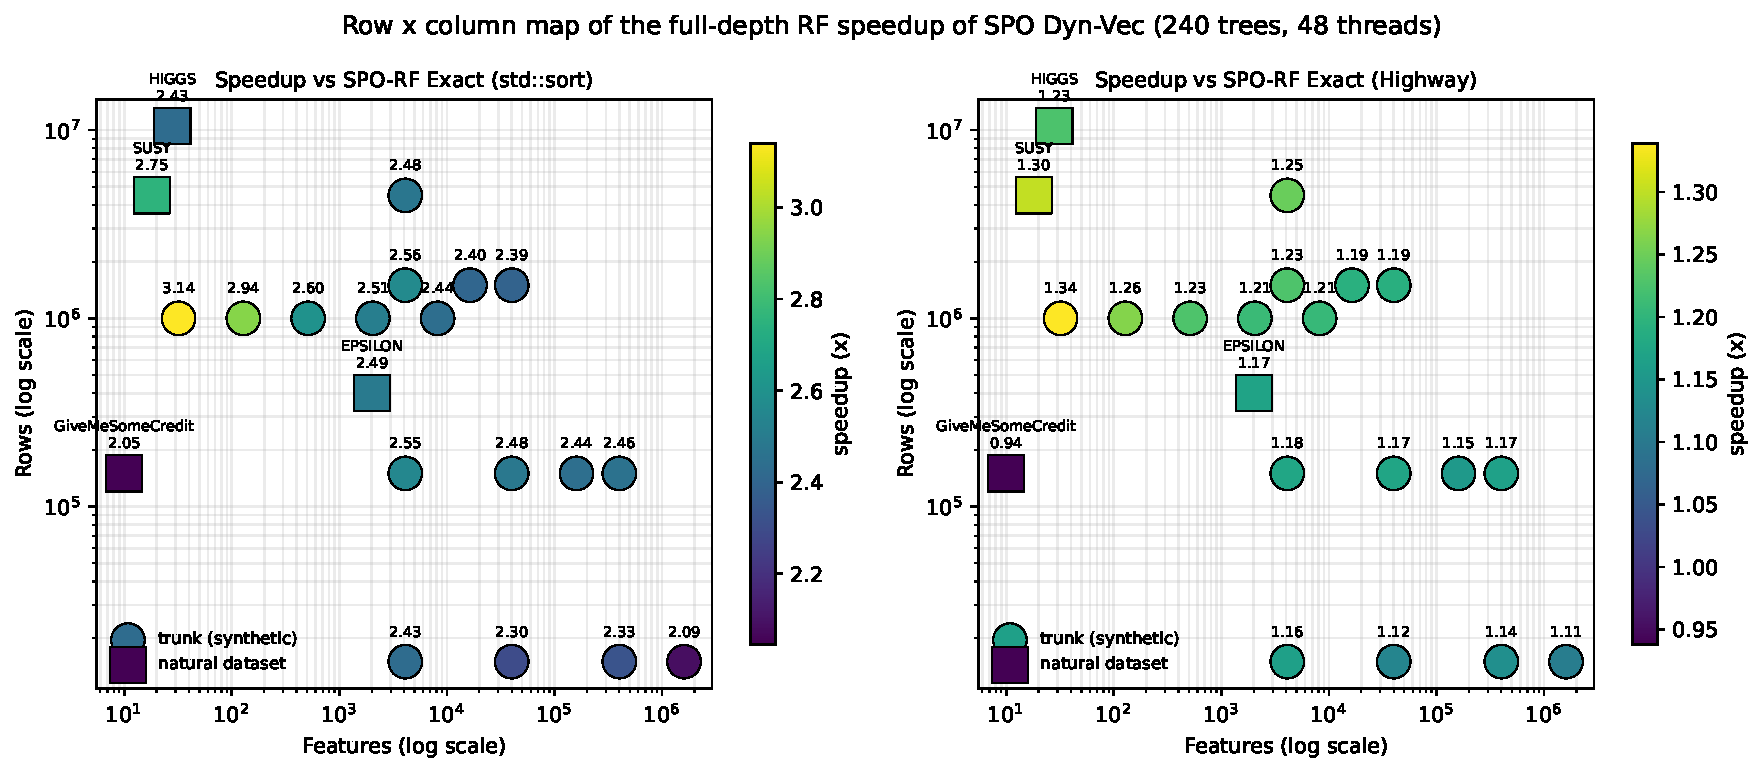
\includegraphics[width=\linewidth]{figures/results/spo_vs_gbt_rowcol_map.pdf}
    \caption{Row $\times$ column map of the full-depth SPO-RF speedup of Dyn-Vec over exact
    splitting with Highway's sort; 240 trees, 48 threads. Circles: Trunk synthetic datasets;
    squares: HIGGS, SUSY, Epsilon and GiveMeSomeCredit. The same map against the
    \texttt{std::sort} baseline is Figure~\ref{fig:rowcol-map-stdsort}.}
    \Description{A scatter panel with features on the x axis and rows on the y axis, both log scale, points colored and annotated by speedup.}
    \label{fig:rowcol-map}
\end{figure}

